%package list
\documentclass{article}
\usepackage[top=3cm, bottom=3cm, outer=3cm, inner=3cm]{geometry}
\usepackage{graphicx}
\usepackage{url}
%\usepackage{cite}
\usepackage{hyperref}
\usepackage{array}
%\usepackage{multicol}
\newcolumntype{x}[1]{>{\centering\arraybackslash\hspace{0pt}}p{#1}}
\usepackage{natbib}
\usepackage{pdfpages}
\usepackage{multirow}
\usepackage{multirow}
\usepackage[normalem]{ulem}
\useunder{\uline}{\ul}{}


%%%%%%%%%%%%%%%%%%%%%%%%%%%%%%%%%%%%%%%%%%%%%%%%%%%%%%%%%%%%%%%%%%%%%%%%%%%%
%%%%%%%%%%%%%%%%%%%%%%%%%%%%%%%%%%%%%%%%%%%%%%%%%%%%%%%%%%%%%%%%%%%%%%%%%%%%
\newcommand{\csemail}{vmachacaa@ulasalle.edu.pe}
\newcommand{\csdocente}{MSc. Vicente Enrique Machaca Arceda}
\newcommand{\cscurso}{Compiladores}
\newcommand{\csuniversidad}{Universidad La Salle}
\newcommand{\csescuela}{Escuela Profesional de Ingeniería de Software}
\newcommand{\cspracnr}{01}
\newcommand{\cstema}{Introducción}
%%%%%%%%%%%%%%%%%%%%%%%%%%%%%%%%%%%%%%%%%%%%%%%%%%%%%%%%%%%%%%%%%%%%%%%%%%%%
%%%%%%%%%%%%%%%%%%%%%%%%%%%%%%%%%%%%%%%%%%%%%%%%%%%%%%%%%%%%%%%%%%%%%%%%%%%%


\usepackage[english,spanish]{babel}
\usepackage[utf8]{inputenc}
\AtBeginDocument{\selectlanguage{spanish}}
\renewcommand{\figurename}{Figura}
\renewcommand{\refname}{Referencias}
\renewcommand{\tablename}{Tabla} %esto no funciona cuando se usa babel
\AtBeginDocument{%
	\renewcommand\tablename{Tabla}
}

\usepackage{fancyhdr}
\pagestyle{fancy}
\fancyhf{}
\setlength{\headheight}{30pt}
\renewcommand{\headrulewidth}{1pt}
\renewcommand{\footrulewidth}{1pt}
\fancyhead[L]{\raisebox{-0.2\height}{
\includegraphics[width=3cm]{img/logo_salle}}}
\fancyhead[C]{}
\fancyhead[R]{\fontsize{7}{7}\selectfont	\csuniversidad \\ \csescuela \\ \textbf{\cscurso} }
\fancyfoot[L]{MSc. Vicente Machaca}
\fancyfoot[C]{\cscurso}
\fancyfoot[R]{Página \thepage}







\begin{document}
	
	\vspace*{10px}
	
	\begin{center}	
		\fontsize{17}{17} \textbf{ Práctica \cspracnr}
	\end{center}
	%\centerline{\textbf{\underline{\Large Título: Informe de revisión del estado del arte}}}
	%\vspace*{0.5cm}
	

	\begin{table}[h]
		\begin{tabular}{|x{4.7cm}|x{4.8cm}|x{4.8cm}|}
			\hline 
			\textbf{DOCENTE} & \textbf{CARRERA}  & \textbf{CURSO}   \\
			\hline 
			\csdocente & \csescuela & \cscurso    \\
			\hline 
		\end{tabular}
	\end{table}	
	
	
	\begin{table}[h]
		\begin{tabular}{|x{4.7cm}|x{4.8cm}|x{4.8cm}|}
			\hline 
			\textbf{PRÁCTICA} & \textbf{TEMA}  & \textbf{DURACIÓN}   \\
			\hline 
			\cspracnr & \cstema & 3 horas   \\
			\hline 
		\end{tabular}
	\end{table}
	
	
	\section{Datos de los estudiantes}
	\begin{itemize}
		\item Grupo: xxxxxx
		\item Integrantes: 
		\begin{itemize}
			\item Kevin Linares Salinas
		\end{itemize}		
		\item Url Github: \url{https://github.com/kjoel2001/Compiladores}
	\end{itemize}
	
	
	

	
	\section{Ejercicios}\label{sec:ejercicios}
	\begin{enumerate}
		\item Redacta el siguiente código, genera con ensamblador y explica en qué parte (del código ensamblador) se definen las variables c y m. (2 puntos).
		
		Solución: \\
		\begin{center}
		    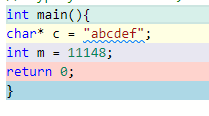
\includegraphics[width=.3\textwidth]{Imagenes/ejercicio 1.1.png}
		    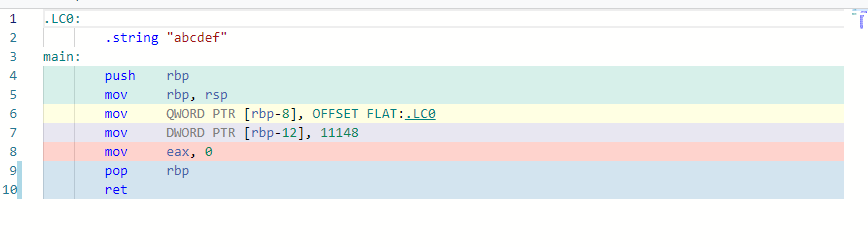
\includegraphics[width=.9\textwidth]{Imagenes/ejercicio 1.png}
		\end{center}\newpage
		\item Redacta el siguiente código, genera el código ensamblador y explica en qué parte (del código ensamblador) se define la división entre 8. (2 puntos).
		
		Solución: \\
        \begin{center}
		    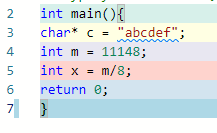
\includegraphics[width=.6\textwidth]{Imagenes/ejercicio 2.png}
		    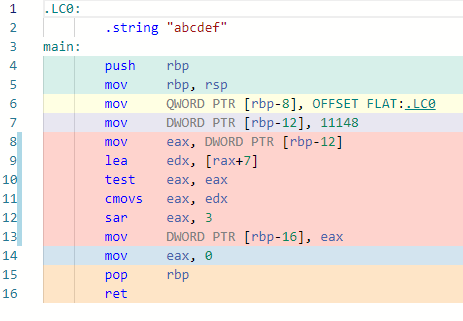
\includegraphics[width=.9\textwidth]{Imagenes/ejercicio 2.1.png}
		\end{center}\newpage

        \item Redacta el siguiente código, genera el código ensamblador y explica en que parte (del código ensamblador) se define la división entre 7. (2 puntos).
        Solución: \\
        \begin{center}
		    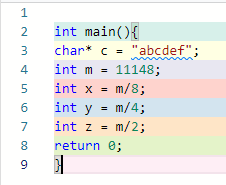
\includegraphics[width=.4\textwidth]{Imagenes/ejercicio 3.png}
		    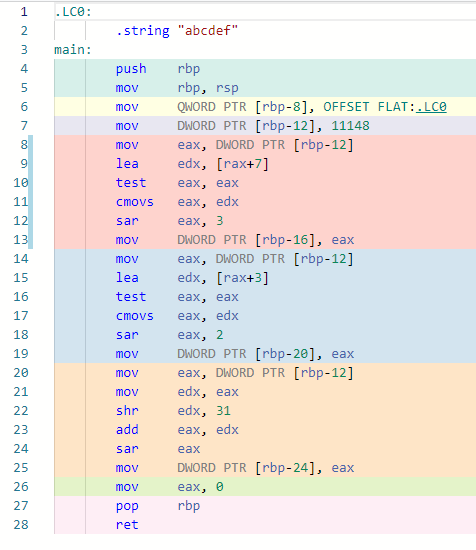
\includegraphics[width=.7\textwidth]{Imagenes/ejercicio 3.1.png}
		\end{center}\newpage
        \item Redacta el siguiente código, genera el código ensamblador y explica en que parte (del código
        ensamblador) se define la división entre 2. (2 puntos).
        Solución: \\
        \begin{center}
		    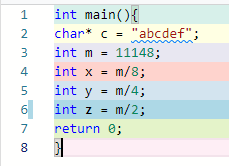
\includegraphics[width=.4\textwidth]{Imagenes/ejercicio 4.png}
		    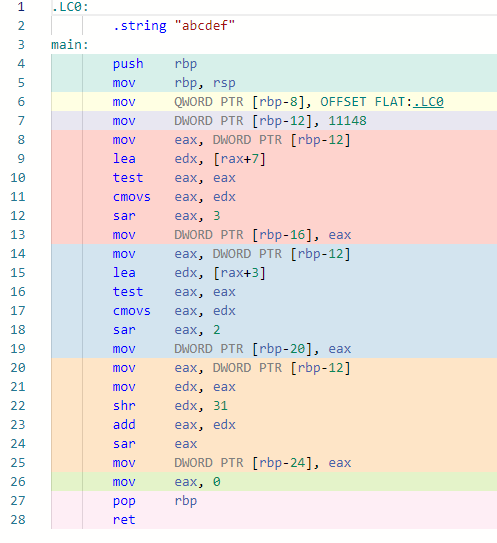
\includegraphics[width=.7\textwidth]{Imagenes/ejercicio 4.1.png}
		\end{center}\newpage
		
        \item Redacta el siguiente código, genera el código ensamblador y explica: (4 puntos):
        \begin{center}
            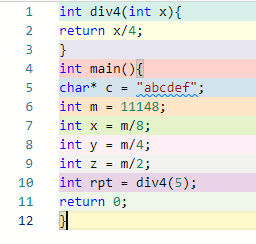
\includegraphics[width=.3\textwidth]{Imagenes/ejercicio 5.png}
            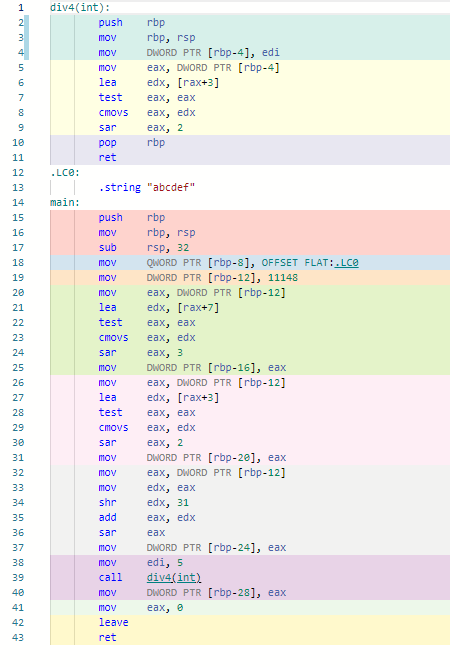
\includegraphics[width=.6\textwidth]{Imagenes/ejercicio 5.1.png}
        \end{center}
        \begin{enumerate}
            \item En que parte del código ensamblador se define la función div4.
                \begin{center}
		              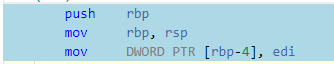
\includegraphics[width=.7\textwidth]{Imagenes/ejercicio 5 a.png}
		        \end{center}
            \item En que parte del código ensamblador se invoca a la función div4.
                \begin{center}
		              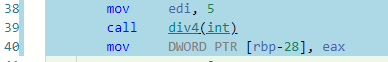
\includegraphics[width=.7\textwidth]{Imagenes/ejercicio 5 b.png}
		        \end{center}\newpage
            \item En que parte del código ensamblador dentro de la función div4 se procesa la división.
                \begin{center}
		              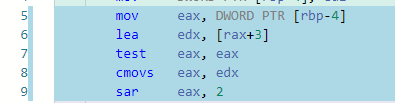
\includegraphics[width=.7\textwidth]{Imagenes/ejercicio 5 c.png}
		        \end{center}
        \end{enumerate} 

        \item Redacta el siguiente código, genera el código ensamblador y explica: (4 puntos):
            \begin{center}
                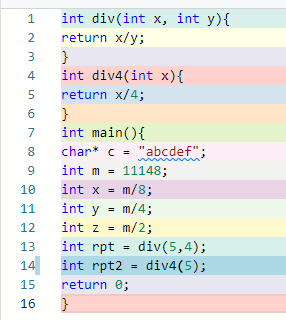
\includegraphics[width=.3\textwidth]{Imagenes/ejercicio 6.png}
                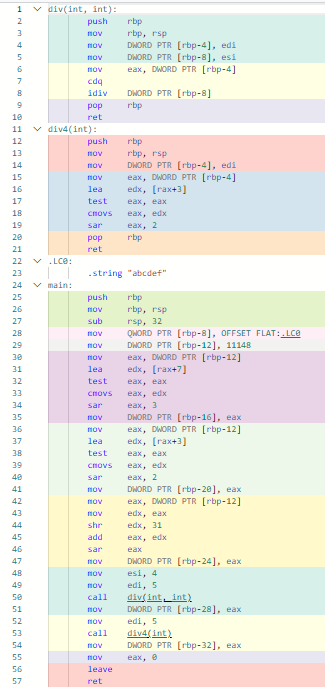
\includegraphics[width=.5\textwidth]{Imagenes/ejercicio 6.1.png}
            \end{center}\newpage
        \begin{enumerate}
            \item En que parte del código ensamblador se define la función div.
            \begin{center}
		              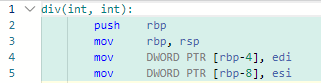
\includegraphics[width=.7\textwidth]{Imagenes/ejercicio 6 a.png}
		        \end{center}
            \item En que parte del código ensamblador se invoca a la función div.
            \begin{center}
		              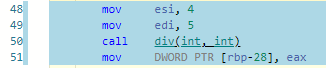
\includegraphics[width=.7\textwidth]{Imagenes/ejercicio 6 b.png}
		        \end{center}
            \item En que parte del código ensamblador dentro de la función div se procesa la división.
            \begin{center}
		              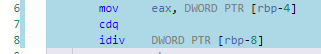
\includegraphics[width=.7\textwidth]{Imagenes/ejercicio 6 c.png}
		        \end{center}
        \end{enumerate} 

        \item De las preguntas anteriores, se ha generado código por cada función, ambas dividen entre 4, pero difieren un poco en su implementación. Investigue a que se debe dicha diferencia y comente cuales podrıan ser las consecuencias. (4 puntos)
	\end{enumerate}


	
	%\clearpage
	%\bibliographystyle{apalike}
	%\bibliographystyle{IEEEtranN}
	%\bibliography{bibliography}
		
	
\end{document}